\documentclass{article}
\usepackage{amsmath}
\usepackage{amssymb}
\usepackage{amsthm}
\usepackage{empheq}
\usepackage[most]{tcolorbox}
%\usepackage[a4paper, total={6in, 8in}]{geometry}
\usepackage[a4paper,bindingoffset=0.2in,%
            left=1in,right=1in,top=1in,bottom=1in,%
            footskip=.25in]{geometry}
\usepackage{algorithm}
\usepackage[noend]{algpseudocode}
%\usepackage[francais]{babel}
\usepackage{listings}
\usepackage[utf8]{inputenc}
\usepackage[T1]{fontenc}
\usepackage{subcaption}



\makeatletter
\def\BState{\State\hskip-\ALG@thistlm}
\makeatother

\usepackage{import}
\usepackage{xifthen}
\usepackage{pdfpages}
\usepackage{transparent}
\usepackage{caption}
\usepackage{subcaption}
\usepackage{hyperref}

\captionsetup[subfigure]{labelformat=empty}

\newcommand{\incfig}[1]{%
    \colorbox{white}{
        \def\svgwidth{\columnwidth}
        \import{./figures/}{#1.pdf_tex}
    }
}

\newtheorem{definition}{Definition}
\newtheorem{proposition}{Proposition}
\newtheorem{theorem}{Theorem}
\author{Pierre Glaser, Clement Chadebec}
\title{Rapport de projet - Geodesic Methods and Deformable Models}
\begin{document}
\maketitle
\pagebreak
%\vspace*{-10em}
\part*{Questions}


\paragraph{Quel est le problème traité?} 
Nous étudierons dans ce rapport l'article \emph{Template Matching via densitives on the
Roto Translation Group}, par Erik J. Bekkers et. Al. \cite{main}

Le problème traité est la \textbf{localisation} d'un objet d'intérêt dans une image par
\textbf{apprentissage supervisé}. Dans les jeux de
données utilisés, l'objet est par exemple le disque optique d'un œil, ou bien la
rétine. Un des présupposés majeurs de l'article est que les problèmes en question bénéficieraient d'une prise en
compte des structures d'orientation locale en tout point de l'image.

\paragraph{Quelles sont les équations et les méthodes numériques utilisées?} 
\begin{itemize}
    \setlength{\itemsep}{0pt}
    \item La localisation de l'objet d'intérêt dans une image se fait par
      \emph{cross-correlation} \cite{cross-correlation}: un
        \emph{template} est ``appliqué`` en tout point $ x $ de l'image.  La valeur
        maximale du résultat est alors la localisation prédite de l'objet. Formellement,
        si $ f $ est l'image, et $ x $ le template:
      \[
      {x}^{\star} = \arg \max_{ \tilde{ x } } \langle  f, \mathcal  T_{ \tilde{ x }}
      t\rangle_{L_2(\mathbb{R}^2)}
      \] 
      ou $ \mathcal  T_{ \tilde{ x }}$  est l'opérateur translation, défini comme
      \[
      \begin{aligned}
        T_{ \tilde{ x }}t:  \mathbb{R}^2 &\longrightarrow \mathbb{R}^2 \\
                                         &\longmapsto \left ( T_{ \tilde{ x }}t \right )(x) = t( x - \tilde{ x })
      \end{aligned}
      \] 
       est l'opérateur translation.
    \item Dans le cas standard exposé ci-dessus, $ f $ est définie sur $ \mathbb{R}^2 $. Cependant, $ f $
        peut être transformée (e.g relevée, soulevée) depuis $ \mathbb{R}^2  \to
        \mathbb{R} $  vers $ \mathbb{R}^2 \times \lbrack 0, 2 \pi \rbrack  \to \mathbb{
        C} $, ou autrement dit, $ SE2(\mathbb{R}) $. La dimension
        additionnelle décrit en chaque point l'état local de l'orientation de l'image
        selon un certain nombre de directions.
    \item Afin d'obtenir des bonnes performances en prédiction, le template $ t $ est
      défini comme solution d'un problème d'optimisation de type
        moindres carrés régularisés, ou régression logistique régularisée.
        Typiquement,
        \[
        t = \arg \min_{  } \sum\limits_{ i=1 }^{ N } \left ( \langle t, p_i \rangle
        - y_i \right )^2 + R(t) 
        \] 
        les $ p_i $ sont des templates individuels ``idéaux'': ce sont des patches,
        extraits des images, de la même taille que $ t $ . Si ils sont centrés en le point d'intérêt
        de l'image $ i $, ce sont des patches dits ``positifs`''. Les patchs ne correspondant à aucune zone d'intérêt 
        dans l'image sont dit ``négatifs''. Les $y_i$ correspondent aux labels et on a $y_i =1$ si le patch est 
        postif (i.e. une zone d'intérêt y est présente), $y_i=0$ sinon. Si l'on suppose que 
        \begin{itemize}
            \item $ \|p_i\| = 1 $
            \item n'importe quelle coupe de $ f_i $, une image, de la taille de $ p_i $ a une norme
                de $ 1 $
        \end{itemize}
        on a $ (p_i \star f_i)(x) = \mathcal  \langle T_x(p_i) f_i[p_i] \rangle  \leq
        \|p_i\| \|f_i[p_i]\| \leq  1$, le maximum étant atteint quand $ f_i $ et $ p_i $ 
        sont alignés, ceci arrivant par construction en $ {x}^{\star}_i $
        ou 
    \item $ R(t) $ est une pénalité imposant de la régularité à t. Elle contient deux
      termes dont le poids peut être modulé:
      \begin{itemize}
        \item un terme de robustesse de type $ \mu\|t\|^2 $,
        \item un terme de ``smoothness'' de type $ \int\limits_{  }^{  } \| \nabla_{
          } t \|^2 d \mu $
      \end{itemize}
    \item A ce moment là, le template est une variable dans $ \mathbb{R}^N$, N étant le
      nombre de pixels du patch (Typiquement, le patch est de dimension bien
        inférieure à celle des images entières). On pourrait alors optimiser chaque pixel
        respectivement, mais il serait alors difficile de formuler les contraintes de
        ``smoothness'' du patch final. Une autre manière de faire est de paramétriser le
        patch comme une combinaison linéaire de fonctions régulières: c'est l'approche
        suivie dans cet article, qui utilise comme fonctions les B-splines \cite{bspline}. Le template
        s'écrit alors
        \[
            t(x, y) = \sum\limits_{ k=1 }^{ N_k } \sum\limits_{ l=1 }^{ N_l } c_{k, l} B^n \left (
            \frac{x}{s_k} - k \right ) B^n \left ( \frac{y}{s_{l}} - l \right )
            \label{eq:spline} \tag{1}
        \] %
        %\vspace*{-1em}
        ($ s_k $ et $ s_l $ sont des paramètres d'échelles fixés au préalable: il
        ne sont pas des fonctions des indices $ k $ et $ l $).
        Une expression qui admet alors un gradient, ceci permettant d'obtenir une
        formulation du terme: 
        \[
            \int\limits_{  }^{  } \| \nabla_{  } t(x, y) \|^2 dx dy
        \] 
    \item \vspace*{-1.5em} Toutes ces formulations et paramétrisations sont pour l'instant uniquement
      valables pour les images dans leur forme initiale (non soulevées). Un
      investissement supplémentaire est nécessaire pour reformuler le problème
      d'optimisation ainsi que les pénalités de régularisation pour optimiser un
      template "soulevé". Ces équations seront étudiées plus en détail dans la section
      \ref{part:details}
\end{itemize}

\paragraph{Pouvez vous situer l'article par rapport aux méthodes étudiées en cours et le
comparer à des sujets proches évoqués en cours?} 
La différence principale avec les sujets étudiés en cours est que cette méthode est une
méthode d'apprentissage supervisée et automatique alors que les méthodes étudiées
pendant le cours sont non supervisées et demandent généralement une intervention humaine
au moment de l'initialisation.\newline
Une caractéristique commune de ces deux méthodes est la présence d'un terme de
pénalisation sur la régularité de la solution du problème d'optimisation, les deux
faisant intervenir le gradient le la paramétrisation: on rappelle que le problème des
contours actifs s'écrit:
\[
    \int\limits_{  \Omega }^{  } \left ( w_1^2 \|C'(s)\|^2 + w_2^2 \|C''(s)\|^2 +
    P(C(s)) \right )ds
\] 
alors que le problème étudié concerne la résolution de 
\[
    t = \arg \min_{  } \sum\limits_{ i=1 }^{ N } \left ( \langle t, p_i \rangle
    - y_i \right )^2 + \lambda \int\limits_{  }^{  } \| \nabla_{  } t(x, y) \|^2 dx dy + \mu \| t \|^2
    \label{eq.2} \tag{2}
\]
\paragraph{Quelle est l'originalité du travail (selon les auteurs)?}
Ce travail s'inscrit dans la continuité d'une  série d'article des auteurs: la majorité
des concepts utilisés dans cet articles on été introduits dans des publications
précédentes:
\begin{itemize}
  \item l'utilisation des scores d'orientation a été introduit en \cite{orientation-score}
  \item les cake wavelets ont été introduites dans \cite{cake}
  \item la cross-corrélation est une technique bien connue pour détecter des points
    d'intérêts \cite{cross-correlation}.
\end{itemize}
Les auteurs proposent alors une méthode de résolution pour une reformulation de la 
``regression logistique'' permettant à cette méthode d'atteindre l'état de l'art en
termes de performances, ainsi qu'une série d'expériences très complètes
comparant l'influence des différents types de régularisation et l'importance des
scores d'orientation. Enfin, est donnée en appendice une interprétation mathématique d'une
version simplifiée du problème régularisé dans $ SE2(\mathbb{R}) $
\paragraph{Quels sont les résultats nouveaux importants qui en découlent?}
Le résultat le plus important ici est à nos yeux la preuve expérimentale que cette
méthode atteint l'état de l'art pour les jeux de données considérées.
\paragraph{Voyez vous des faiblesses dans l'approche présentée et avez-vous des idées
pour y faire face?}
Une faiblesse de la méthode proposée selon nous est que cette méthode semble peu robuste
aux changements d'échelle (détails expérimentaux dans \ref{part:details}), quelque chose qui est très fréquent dans les jeux de données
d'images. Pour y remédier, on pourrait considérer une base d'ondelettes plus riches,
pouvant prendre en compte différents types d'échelles, mais pour être admissible, une
ondelette doit satisfaire un cahier des charges fourni (voir plus tard les détails
théoriques sur les ondelettes de cake).  Il n'est donc pas simple (mathématiquement) de
changer d'ondelettes pour rendre la méthode invariante aux changements d'échelle.


\part{Rapport détaillé}\label{part:details}
\section{Discussions théoriques}
Nous rentrons maintenant plus en détail dans les notions spécifiques à l'article, à
savoir le soulèvement dans l'espace des scores d'orientations, et la redéfinition du
template-matching et du problème d'optimisation associé dans cet espace.
\paragraph{Les scores d'orientation} 
Un concept majeur du papier concerne la manière de prendre en compte l'état
d'orientation de chaque point de l'image afin de mieux détecter le point d'intérêt.
L'approche consiste a convoluer l'image avec le $ R_{\theta} \phi $, ou $ R_{\theta} $
est la rotation d'angle $ \theta  $, et $ \phi $ est une ondelette.
l'image 
\[
    \begin{aligned}
        f: \mathbb{R}^2 &\longrightarrow \mathbb{R} \\
        (x, y) &\longmapsto f(x, y)
    \end{aligned}
\] 
devient alors 
\[
\begin{aligned}
    U_f: \quad \mathbb{R}^2\times \lbrack  0, 2 \pi \rbrack &\longrightarrow \mathbb{C} \\
    (x, y, \theta) &\longmapsto U_f(x, y, \theta)
\end{aligned}
\] 
$ \theta $, tout comme $ x $ et $ y $ est discrétisé.
La construction de ce score d'orientation est inspirée par le fonctionnement du cortex
visuel des mammifères \cite{cake2}.
On effectue alors un certain nombre de remarques sur cette transformée
\begin{itemize}
    \item Par definition, $  U_f $ est une transformée en ondelettes:
        \[
             U_f(g) =  (\mathcal W_{\phi}[f])(g)  = \langle \mathcal  U_g \phi, f
             \rangle_{\mathbb{R}^2}
        \] 
        et $ \mathcal  U_g $ est une representation:
        \[
            \mathcal  U_g \phi(x) = (\mathcal  T_b \mathcal  R_{e^{i \theta}} \phi )(x)
            = \phi \left ( R_{\theta}^{-1}(x - b) \right )
        \] 
        \item $ f  \to U_f $ transforme $ L_2(\mathbb{R}) $ en un espace de Hilbert $
        \mathbb C_K^{\mathbb{R}^2 \times \mathbb{ T }} $.\newline
        Tout comme la transformée de Fourier (aux constantes multiplicatives près), la
        transformation $ U_f $ est une isométrie:
        \[
            \|f\|_{L_2(\mathbb{R})} = \|U_f\|_{M_{\phi}}
        \] 
        où $ M_{\phi} $ est une fonction caractérisant le produit scalaire de cet espace
        de Hilbert.\newline
        De cette propriété découle l'inversibilité de la transformée en scores
        d'orientation.
        \item Contrairement à la transformée en ondelettes classique, cette transformée
            ne fait pas intervenir différentes échelles, ce qui dans les cas étudiés,
            semble être considéré comme quelque chose de désirable dans les articles la
            décrivant, mais qui peut s'avérer néfaste dans notre cas (voir \ref{paragraph:robustness-to-scale}) 
        \item La stabilité de la transformée inverse est complètement déterminée par la
            fonction $ M_{\phi} $; c'est sous ce critère que l'ondelette de base $ \phi
            $ est choisie.
\end{itemize}
Les ondelettes ``cake'' (gateau en anglais) s'avèrent avoir un $ M_{\phi} $ optimal, et
être d'excellents détecteurs de lignes. Le nom de ces ondelettes provient du fait que
dans le plan de fourrier, le support de l'ondelette ressemble a une part de gateau.
C'est cette ondelette qui a été choisie comme base pour créer les scores d'orientation
dans le papier étudié.
\vspace{5em}
\begin{figure}[htpb]
\centering
\hspace*{-6em}
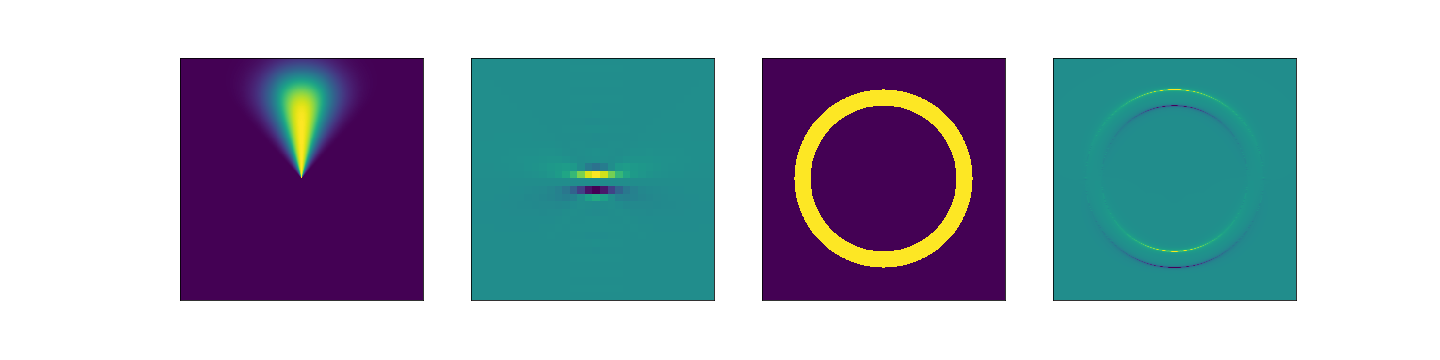
\includegraphics[scale=0.39]{plots/cake_wavelet.png}
\caption {Simulation personnelles des ondelettes de  cake}
de gauche à droite: l'ondelette dans le plan de fourrier, l'ondelette dans le domaine
spatial, une image simple, et la même image transformée par cette ondelette.
\end{figure}

\paragraph{Extension à $SE(2)$}
Comme présenté au dessus, le score d'orientation permet de capturer d'une certaine manière les axes dominants d'un image dans une certaine direction. De ce fait, 
l'utilisation de ce score semble être d'intérêt pour des problèmes de détection.
Dans, ce papier les auteurs ont ainsi fait le choix d'étendre le problème d'optimisation comme présenté en \ref{eq.2} à $SE(2)$ via 
l'utilisation du score d'orientation. 
\begin{itemize}
  \item La notion de cross-correlation est étendue naturellement a $ SE(2) $
\end{itemize}
Il s'agit désormais de s'intéresser au problème d'optimisation étendu:
\[
  \sum \limits_{i=1}^N (\langle t, |U_{fi}| \rangle_{{\mathbb{L}_2(SE(2))}} - y_i)^2 + \lambda \int \limits_{\mathbb{R}^2} \int \limits_{0}^{2\pi} \lVert 
  \nabla t(x, y, \theta)\rVert_{D}^2 dxdyd\theta + \mu \lVert t \rVert_{\mathbb{L}_2(SE(2))}^2
\]
Les $U_{fi}$ sont les scores d'orientation des patchs $p_i$.
Le produit scalaire définit sur $SE(2)$ prend la forme suivante:
\[
    \langle t, |U_{fi}| \rangle_{SE(2)} = 
    \int \limits_{\mathbb{R}^2} \int \limits_{0}^{2\pi} \overline{t(x, y, \theta)} \lvert U_f (x, y, \theta) \rvert dxdyd\theta
\]

Et $\nabla t$ est le gradient invariant à gauche déduit des dérivées partielles invariantes à gauches définies sur $SE(2)$
comme suit $\{\partial_{\xi} = cos(\theta)\partial_x + sin(\theta) \partial_y,\, \partial{\eta} = -sin(\theta) \partial_x + cos(\theta)
\partial_y, \partial_{\theta}\}$. Une norme pondérée du gradient peut ensuite être définie comme suit:
\[
    \lVert \nabla t \rVert_{D}^2 = D_{\xi \xi} \Big|\frac{\partial t}{\partial \xi} \Big|^2
    + D_{\eta \eta} \Big|\frac{\partial t}{\partial \eta}\Big|^2 + D_{\theta \theta} \Big|\frac{\partial t}{\partial \theta}\Big|^2
\]


Les paramètres $D_{\xi \xi}, D_{\eta, \eta}$ et $D_{\theta \theta}$ sont des paremètres de régularisation permettant de 'pénaliser' ou 'favoriser' une certaine direction.
De manière identique à l'approche employée dans $\mathbb{R}^2$, le template final est paramétré par une famille de fonctions
régulières telles que les B-splines étendues à $SE(2)$.
\[
    t(x, y, \theta) = \sum \limits_{k=1}^{n_k} \sum \limits_{l=i}^{N_l} \sum \limits_{m=1}^{N_m} c_{k,l,m} B^n \left (\frac{x}{s_k} - k \right )
    B^n \left (\frac{y}{s_l} - l \right) B^n \left (\frac{\theta \text{mod} 2\pi}{s_m} - m \right )
\]

\paragraph{Regression logistique}
Dans les deux espaces considérés, $\mathbb{R}^2$ et $SE(2)$, un modèle de regression logistique est également proposé en comparaison 
au modèle de régression linéaire. Dans les problèmes de détection, le but majeur est de séparer les patches $f_i$ correspondant aux zones d'une image correspondant à une 
zone d'intérêt ($y_i =1$) des zones sans objet ($y_1=0$). Cependant, une approche différente de \ref{eq.2} et ne faisant pas intervenir le terme de perte quadratique 
peut être également employée. Ici, les auteurs ont décidé d'avoir recours à un modèle de régression logistique dans lequel la présence ou non de 
la zone d'intérêt au sein d'un patch $f_i$ est représentée par une certaine probabilité de présence $p_i$. Cette probabilité est inférée à l'aide de
la function ``sigmoide'' telle que $p_i = \sigma(\langle t, f_i \rangle)$. Le le but revient à trouver le template qui maximise la vraisemblance $l(t) = 
\prod \limits_{i=1}^N p(f_i; t)^{y_i}(1 - p(f_i; y))^{1- y_i}$
des patches $f_i$ étant donnés leurs labels $y_i$. Dans une telle approche la log-vraissemenblance permet de 'linéariser' le problème d'optimisation qui prend la forme
suivante dans $\mathbb{R}^2$:
\[
    \arg \max \sum \limits_{i=1}^N \langle t, f_i \rangle_{\mathbb{L}_2(\mathbb{R}^2)} - \log \left ( 1 + e^{\langle t, f_i \rangle_{\mathbb{L}_2(\mathbb{R}^2)}}\right) - \lambda \int \limits_{\mathbb{R}^2} \lVert \nabla 
    t \rVert_{\mathbb{L}_2(\mathbb{R}^2)}^2 dx dy - \mu \lVert t \rVert_{\mathbb{L}_2(\mathbb{R}^2)}^2
\]
ou dans $SE(2)$:
\[
    \arg \max \sum \limits_{i=1}^N \langle t, |U_{f_i}| \rangle_{\mathbb{L}_2(SE(2))} - \log \left ( 1 + e^{\langle t, |U_{f_i}| \rangle_{\mathbb{L}_2(SE(2))}}\right) - \lambda \int \limits_{\mathbb{R}^2} \int \limits_{0}^{2\pi}\lVert \nabla 
    t \rVert_{D}^2 dx dy d\theta- \mu \lVert t \rVert_{\mathbb{L}_2(SE(2))}^2
\]

\paragraph{Prepocessing des images}
Les jeux de données utilisés sont composés d'images démontrant de forte variation de luminosité et de contraste. Ainsi, une 
phase de \textit{preprocessing} est nécessaire afin de renormaliser les images. La méthode employée dans l'article et que nous 
avons également recodée pour réaliser les expériences décrites plus bas se fonde sur l'idée de renormalisation locale et tirée de \cite{preprocessing}. Elle consiste
à premièrement calculer une moyenne et un écart-type local de l'intensité des pixels. Ceci permet de renormaliser localement l'image afin 
que cette dernière est une moyenne nulle et un écart-type de 1. Ensuite, un masque de fond est extrait en utilisant la distance de Mahalanobis 
permettant d'éviter la prise en compte des valeurs abhérantes dans la seconde phase de normalisation. L'image est ensuite renormalisée une seconde 
fois mais en ignorant les pixels ajoutés au masque.



\section{Expériences} \label{part:expe}

Afin de mieux comprendre leur fonctionnement et de pouvoir les comparer dans 
divers cadres d'études, nous avons re-codé les différentes méthodes présentées dans cet article 
en langage \textit{python}. Le code complet peut être trouvé au lien suivant ???????
Pour mémoire, 5 types de construction de templates sont envisagés:
\begin{itemize}
    \item A: Template obtenu par moyenne de tous les patches positifs (i.e. centrés sur la zone d'intérêt) et normalisation.
    \item B: Template optimisé sans régularisation ($\mu =0$, $\lambda = 0$)
    \item C: Template optimisé avec $\mu$ ($\lambda=0$)
    \item D: Template optimisé avec $\lambda$ ($\mu = 0$)
    \item E: Template optimisé avec $\mu$ et $\lambda$
\end{itemize}

Pour chacune de ses constructions, un module de regression linéaire et regression logistique est employé dans 
les espaces $\mathbb{R}^2$ et $SE(2)$. Afin de réaliser les expérience dont les résultats sont présentés plus 
ont été réalisée en considérant un ensemble de 500 images dont 80\% (400 images) constitue l'ensemble d'entrainement 
des modèles et les 20 \% (100 images) restants l'ensemble de test.
Sur chacune des images d'entrainement, un patch 
positif de taille $N_x \times N_y = 101 \times 101$ centré autour des coordonnées de l'œil gauche et un patch négatif 
de même de taille tiré aléatoirement en dehors des zones d'intérêts (œil droit et gauche) sont crées. Une détection est 
ensuite considérée "bonne" sur le point de détection se situe dans rayon de $10$ pixels autour de la position réelle de l'œil 
gauche. Le nombre de splines considéré est de $N_k = 51$ , $N_l =51$ et $N_m = 4$.



\paragraph{Template Matching dans $\mathbb{R}^2$}
Premièrement, une comparaison des résultats obtenus avec les différentes méthodes a été réalisée dans $\mathbb{R}^2$.
Les résultats sont reportés dans \ref{table: R2}. Afin de trouver les valeurs optimales de $\mu$ (resp $\lambda$) dans les expériences C (resp. D), nous avons décidé 
de procéder de façon empirique en faisant varier les valeurs de ces deux paramètres entre $10^{-4}$ et $1$. Afin de trouver le meilleur couple pour l'expérience E, nous avons 
choisi de tout d'abord fixer la valeur de $\mu$ et $\lambda$ à leur valeur optimale
trouvée lors des expériences C et D $ {\mu}^{\star}$ et $ {\lambda}^{\star}$, puis de faire légèrement leurs valeurs autour de ces optimaux.
Il s'est avéré que comme présenté dans l'article un choix de couple $\mu = 0.5
{\mu}^{\star}$ et $\lambda = 0.5 {\lambda}^{\star}$ fournissait les meilleurs résultats.

\begin{table}[h!]
    \centering
    \begin{tabular}{|c|c|c|}
        \hline
        Méthode & Score (\%)\\
        \hline
        \hline
        $A^{\mathbb{R}^2}$& 61.0 \% \\
        \hline
        $B_{\text{lin}}^{\mathbb{R}^2}$& 3.0 \%    \\
        $C_{\text{lin}}^{\mathbb{R}^2}$& 62.0 \%   \\
        $D_{\text{lin}}^{\mathbb{R}^2}$& 38.0 \%   \\
        $E_{\text{lin}}^{\mathbb{R}^2}$& 62.0 \%   \\
        \hline
        $B_{\text{log}}^{\mathbb{R}^2} $& 0.0 \%   \\ 
        $C_{\text{log}}^{\mathbb{R}^2} $& 63.0 \%  \\ 
        $D_{\text{log}}^{\mathbb{R}^2} $& 26.0 \%   \\ 
        $E_{\text{log}}^{\mathbb{R}^2} $& 63.0 \%  \\ 
        \hline
    \end{tabular}
    \caption{Résultats obtenus par template matching dans $\mathbb{R}^2$}
    \label{table: R2}
\end{table}

La table \ref{table: R2} montre qu'un template relativement simple ne correspondant finalement qu'à la moyenne de tous les patches positifs démontre tout de même de bons
résultats comparé à des modèles de régression plus évolués. Effectivement, si non couplés à de mécanismes de régularisation, les modèles $B_{\text{log}}^{\mathbb{R}^2} $ et 
$B_{\text{lin}}^{\mathbb{R}^2} $ ne démontre que de faibles performances. Par ailleurs, un bon choix de paramètres de régularisation peut conduire à améliorer drastiquement les 
performances des regressions dont le meilleur résultat est observé pour $\mu = 10^{-1}$ et $\lambda = 10^{-2}$ pour la regression linéaire et $\mu = 10^{-1}$ et $\lambda = 10^{-3}$ pour la regression logistique.
C'est deux modèles de regression semblent d'ailleurs démontrer des niveaux de performance similaire.
Le "meilleur" modèle dans $\mathbb{R}^2$ est néanmoins obtenu dans le cas E avec la regression logistique (63\%). Ces résultats semblent alignés avec ceux présentés par les auteurs bien que dans $\mathbb{R}^2$, 
il semble que le patch moyenné $A^{\mathbb{R}^2}$ démontre les meilleurs résultats, les
suivant sont $C_{\text{lin}}^{\mathbb{R}^2}, E_{\text{lin}}^{\mathbb{R}^2},
C_{\text{lin}}^{\mathbb{R}^2}$ et $E_{\text{log}}^{\mathbb{R}^2}$ qui marchent de manière 
similaires.


\paragraph{Template Matching dans $SE(2)$}
Les mêmes expériences ont ensuite été reproduites en utilisant l'espace $SE(2)$ et donc ajoutant également l'orientation score dans les régressions.
Cependant, dans cette section les paramètres le paramètres $\mu \in [10^{-5}, 10^{-1}]$ et $\lambda \in [10^{-4}, 10^{-1}]$. En ce qui concernent les paramètres inhérents à la matrices de 
régularisation ont été fixé comme suit $D_{\xi \xi}=1, D_{\eta \eta} = 0$ et $D_{\theta \theta} = 10^{-2}$. Nous n'avons pas fait varié ces paramètres qui ont été choisis en accord avec les auteurs 
de l'article présenté. Les résultats peuvent être observés en \ref{table: SE(2)}.

\begin{table}[h!]
    \centering
    \begin{tabular}{|c|c|c|}
        \hline
        Méthode & Score (\%)\\
        \hline
        \hline
        $A^{SE(2)}$&  63.0 \% \\
        \hline
        $B_{\text{lin}}^{SE(2)}$&  67.0    \%   \\
        $C_{\text{lin}}^{SE(2)}$&  88.0    \%   \\
        $D_{\text{lin}}^{SE(2)}$&  26.0   \%   \\
        $E_{\text{lin}}^{SE(2)}$&  89.0    \%   \\
        \hline
        $B_{\text{log}}^{SE(2)} $&  7.0  \%   \\ 
        $C_{\text{log}}^{SE(2)} $&  55.0  \%   \\ 
        $D_{\text{log}}^{SE(2)} $&  18.0 \%   \\ 
        $E_{\text{log}}^{SE(2)} $&  53.0  \%   \\ 
        \hline
    \end{tabular}
    \caption{Résultats obtenus par template matching dans $SE(2)$}
    \label{table: SE(2)}
\end{table}

Finalement, les résultats présentés en \ref{table: SE(2)} démontrent l'intérêt de considérer des templates dans un espace étendu tel que $SE(2)$.
Si le template créé par moyenne de tous les patches positifs ne marche que légèrement mieux dans $SE(2)$ (63\% v. 61\%), l'efficacité 
lors de la création de template via des régressions dans $SE(2)$ est remarquable. En effet, une simple régression linéaire sans aucune régularisation permet 
d'atteindre un niveau de performance bien supérieur passant de 3\% dans $\mathbb{R}^2$ à 67\% dans $SE(2)$. Si maintenant, 
un simple régularisation $l-2$ est considérée (cas C), combinée à un choix judicieux de $\mu$,  la performance peut atteindre 88\% de précision.
L'ajout d'un nouveau terme régularisant (cas E) et un bon choix de constante permet d'obtenir le meilleur résultat. Seul le cas D, démontre une 
performance plus faible que le même cas dans $\mathbb{R}^2$ qui était également l'un des moins performants. Les résultats que nous présentons sont en ligne avec ceux 
présentés par les auteurs en ce qui concerne les regressions linéaires. Notre meilleur modèle est dérivé de la méthode $C_{\text{lin}}^{SE(2)}$. Pour 
les regressions logistiques, nos résultats sont un peut décevants en comparaison de ceux présenté par les auteurs. 
En termes de temps de calcul, notre modèle est capable d'effectuer une prédiction en 0.23 s avec le modèle obtenue par la méthode $C_{\text{lin}}^{SE(2)}$.


\begin{figure*}[h!]
    \centering

    \begin{subfigure}[b]{0.3\textwidth}
        \centering
        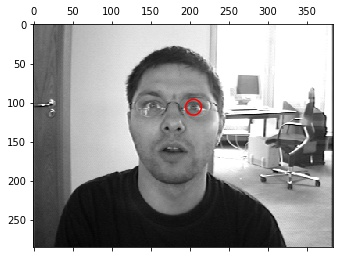
\includegraphics[width=\textwidth]{plots/test_image_detection.jpg}
        \caption{test image}
    \end{subfigure}

    {\small (a)}

    \vskip\baselineskip
    \begin{subfigure}[b]{0.1\textwidth}
        \centering
        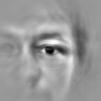
\includegraphics[width=\textwidth]{plots/A_R2_template.jpg}

    \end{subfigure}
    \hspace{-1\baselineskip}
    \vspace{-0.5\baselineskip}
    \quad
    \begin{subfigure}[b]{0.1\textwidth}  
        \centering 
        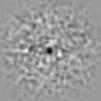
\includegraphics[width=\textwidth]{plots/B_lin_R2_template.jpg}

    \end{subfigure}
    \hspace{-1\baselineskip}
    \quad
    \begin{subfigure}[b]{0.1\textwidth}   
        \centering 
        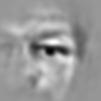
\includegraphics[width=\textwidth]{plots/C_lin_R2_template.jpg}

    \end{subfigure}
    \hspace{-1\baselineskip}
    \quad
    \begin{subfigure}[b]{0.1\textwidth}   
        \centering 
        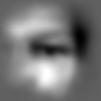
\includegraphics[width=\textwidth]{plots/D_lin_R2_template.jpg}

    \end{subfigure}
    \hspace{-1\baselineskip}
    \quad
    \begin{subfigure}[b]{0.1\textwidth}   
        \centering 
        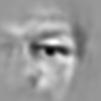
\includegraphics[width=\textwidth]{plots/E_lin_R2_template.jpg}

    \end{subfigure}
    \hspace{-1\baselineskip}
    \quad
    \begin{subfigure}[b]{0.1\textwidth}   
        \centering 
        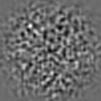
\includegraphics[width=\textwidth]{plots/B_log_R2_template.jpg}

    \end{subfigure}
    \hspace{-1\baselineskip}
    \quad
    \begin{subfigure}[b]{0.1\textwidth}   
        \centering 
        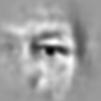
\includegraphics[width=\textwidth]{plots/C_log_R2_template.jpg}

    \end{subfigure}
    \hspace{-1\baselineskip}
    \quad
    \begin{subfigure}[b]{0.1\textwidth}   
        \centering 
        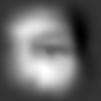
\includegraphics[width=\textwidth]{plots/D_log_R2_template.jpg}

    \end{subfigure}
    \hspace{-1\baselineskip}
    \quad
    \begin{subfigure}[b]{0.1\textwidth}   
        \centering 
        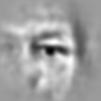
\includegraphics[width=\textwidth]{plots/E_log_R2_template.jpg}

    \end{subfigure}
    \vskip\baselineskip
    \begin{subfigure}[b]{0.1\textwidth}
        \centering
        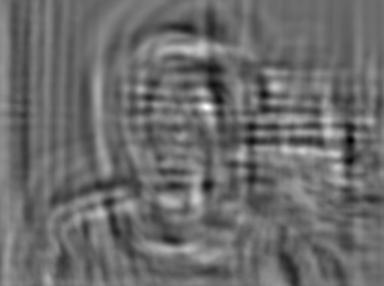
\includegraphics[width=\textwidth]{plots/A_R2_conv.jpg}
        \caption{$A^{\mathbb{R}^2}$}%
        
        \label{fig:mean and std of net14}
    \end{subfigure}
    \hspace{-1\baselineskip}
    \quad
    \begin{subfigure}[b]{0.1\textwidth}  
        \centering 
        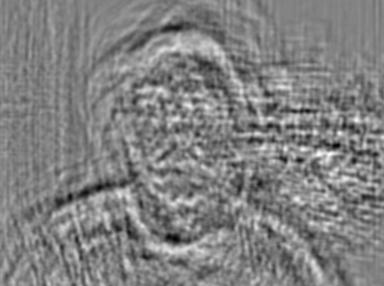
\includegraphics[width=\textwidth]{plots/B_lin_R2_conv.jpg}
        \caption{$B_{\text{lin}}^{\mathbb{R}^2}$}%
         
        \label{fig:mean and std of net24}
    \end{subfigure}
    \hspace{-1\baselineskip}
    \quad
    \begin{subfigure}[b]{0.1\textwidth}   
        \centering 
        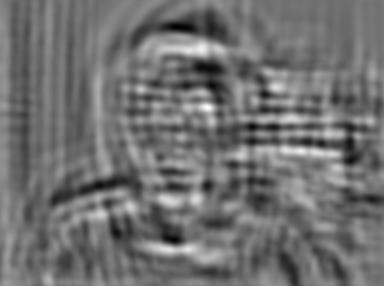
\includegraphics[width=\textwidth]{plots/C_lin_R2_conv.jpg}
        \caption{$C_{\text{lin}}^{\mathbb{R}^2}$}%
           
        \label{fig:mean and std of net34}
    \end{subfigure}
    \hspace{-1\baselineskip}
    \quad
    \begin{subfigure}[b]{0.1\textwidth}   
        \centering 
        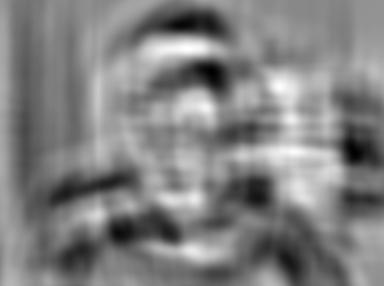
\includegraphics[width=\textwidth]{plots/D_lin_R2_conv.jpg}
        \caption{$D_{\text{lin}}^{\mathbb{R}^2}$}%
        
        \label{fig:mean and std of net44}
    \end{subfigure}
    \hspace{-1\baselineskip}
    \quad
    \begin{subfigure}[b]{0.1\textwidth}   
        \centering 
        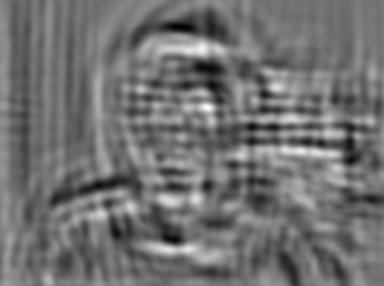
\includegraphics[width=\textwidth]{plots/E_lin_R2_conv.jpg}
        \caption{$E_{\text{lin}}^{\mathbb{R}^2}$}%
        
        \label{fig:mean and std of net44}
    \end{subfigure}
    \hspace{-1\baselineskip}
    \quad
    \begin{subfigure}[b]{0.1\textwidth}   
        \centering 
        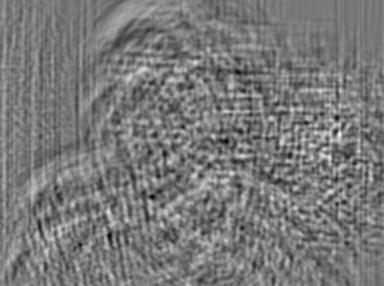
\includegraphics[width=\textwidth]{plots/B_log_R2_conv.jpg}
        \caption{$B_{\text{log}}^{\mathbb{R}^2}$}%
        
        \label{fig:mean and std of net44}
    \end{subfigure}
    \hspace{-1\baselineskip}
    \quad
    \begin{subfigure}[b]{0.1\textwidth}   
        \centering 
        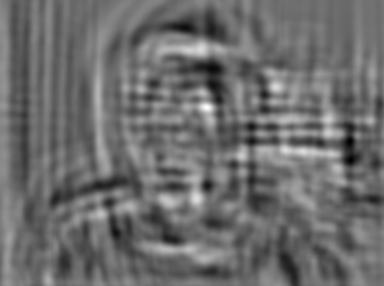
\includegraphics[width=\textwidth]{plots/C_log_R2_conv.jpg}
        \caption{$C_{\text{log}}^{\mathbb{R}^2}$}%
        
        \label{fig:mean and std of net44}
    \end{subfigure}
    \hspace{-1\baselineskip}
    \quad
    \begin{subfigure}[b]{0.1\textwidth}   
        \centering 
        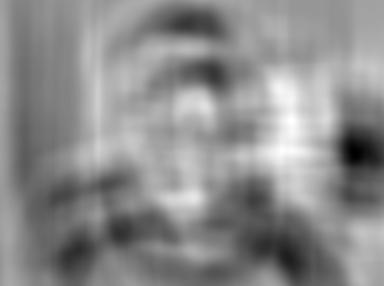
\includegraphics[width=\textwidth]{plots/D_log_R2_conv.jpg}
        \caption{$D_{\text{log}}^{\mathbb{R}^2}$}%
        
        \label{fig:mean and std of net44}
    \end{subfigure}
    \hspace{-1\baselineskip}
    \quad
    \begin{subfigure}[b]{0.1\textwidth}   
        \centering 
        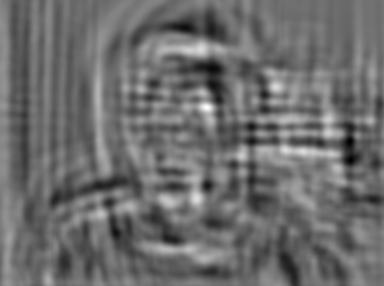
\includegraphics[width=\textwidth]{plots/E_log_R2_conv.jpg}
        \caption{$E_{\text{log}}^{\mathbb{R}^2}$}%
        
        \label{fig:mean and std of net44}
    \end{subfigure}
    {\small (a)}
    \vskip\baselineskip
    \begin{subfigure}[b]{0.1\textwidth}
        \centering
        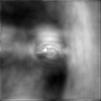
\includegraphics[width=\textwidth]{plots/A_SE2_template.jpg}

    \end{subfigure}
    \hspace{-1\baselineskip}
    \vspace{-0.5\baselineskip}
    \quad
    \begin{subfigure}[b]{0.1\textwidth}  
        \centering 
        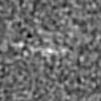
\includegraphics[width=\textwidth]{plots/B_lin_SE2_template.jpg}

    \end{subfigure}
    \hspace{-1\baselineskip}
    \quad
    \begin{subfigure}[b]{0.1\textwidth}   
        \centering 
        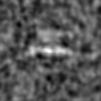
\includegraphics[width=\textwidth]{plots/C_lin_SE2_template.jpg}

    \end{subfigure}
    \hspace{-1\baselineskip}
    \quad
    \begin{subfigure}[b]{0.1\textwidth}   
        \centering 
        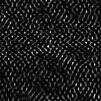
\includegraphics[width=\textwidth]{plots/D_lin_SE2_template.jpg}

    \end{subfigure}
    \hspace{-1\baselineskip}
    \quad
    \begin{subfigure}[b]{0.1\textwidth}   
        \centering 
        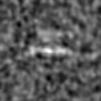
\includegraphics[width=\textwidth]{plots/E_lin_SE2_template.jpg}

    \end{subfigure}
    \hspace{-1\baselineskip}
    \quad
    \begin{subfigure}[b]{0.1\textwidth}   
        \centering 
        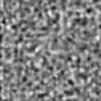
\includegraphics[width=\textwidth]{plots/B_log_SE2_template.jpg}

    \end{subfigure}
    \hspace{-1\baselineskip}
    \quad
    \begin{subfigure}[b]{0.1\textwidth}   
        \centering 
        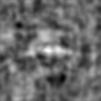
\includegraphics[width=\textwidth]{plots/C_log_SE2_template.jpg}

    \end{subfigure}
    \hspace{-1\baselineskip}
    \quad
    \begin{subfigure}[b]{0.1\textwidth}   
        \centering 
        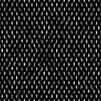
\includegraphics[width=\textwidth]{plots/D_log_SE2_template.jpg}

    \end{subfigure}
    \hspace{-1\baselineskip}
    \quad
    \begin{subfigure}[b]{0.1\textwidth}   
        \centering 
        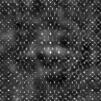
\includegraphics[width=\textwidth]{plots/E_log_SE2_template.jpg}

    \end{subfigure}
    \vskip\baselineskip
    \begin{subfigure}[b]{0.1\textwidth}
        \centering
        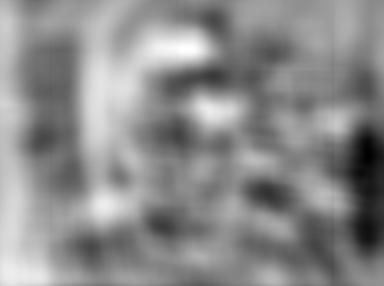
\includegraphics[width=\textwidth]{plots/A_SE2_conv.jpg}
        \caption{$A^{SE(2)}$}%
        
        \label{fig:mean and std of net14}
    \end{subfigure}
    \hspace{-1\baselineskip}
    \quad
    \begin{subfigure}[b]{0.1\textwidth}  
        \centering 
        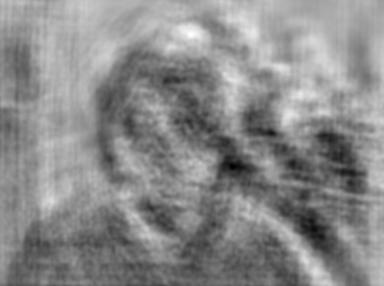
\includegraphics[width=\textwidth]{plots/B_lin_SE2_conv.jpg}
        \caption{$B_{\text{lin}}^{SE(2)}$}%
         
        \label{fig:mean and std of net24}
    \end{subfigure}
    \hspace{-1\baselineskip}
    \quad
    \begin{subfigure}[b]{0.1\textwidth}   
        \centering 
        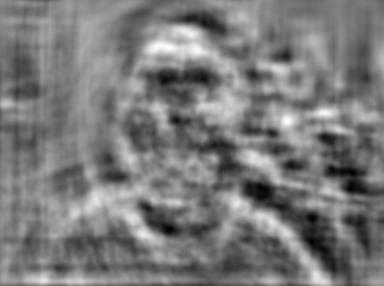
\includegraphics[width=\textwidth]{plots/C_lin_SE2_conv.jpg}
        \caption{$C_{\text{lin}}^{SE(2)}$}%
           
        \label{fig:mean and std of net34}
    \end{subfigure}
    \hspace{-1\baselineskip}
    \quad
    \begin{subfigure}[b]{0.1\textwidth}   
        \centering 
        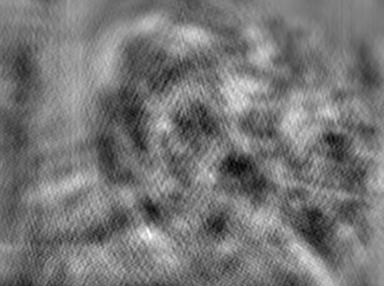
\includegraphics[width=\textwidth]{plots/D_lin_SE2_conv.jpg}
        \caption{$D_{\text{lin}}^{SE(2)}$}%
        
        \label{fig:mean and std of net44}
    \end{subfigure}
    \hspace{-1\baselineskip}
    \quad
    \begin{subfigure}[b]{0.1\textwidth}   
        \centering 
        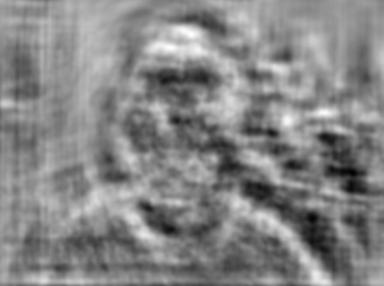
\includegraphics[width=\textwidth]{plots/E_lin_SE2_conv.jpg}
        \caption{$E_{\text{lin}}^{SE(2)}$}%
        
        \label{fig:mean and std of net44}
    \end{subfigure}
    \hspace{-1\baselineskip}
    \quad
    \begin{subfigure}[b]{0.1\textwidth}   
        \centering 
        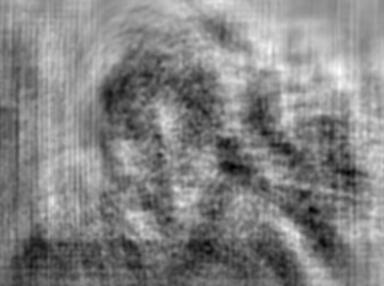
\includegraphics[width=\textwidth]{plots/B_log_SE2_conv.jpg}
        \caption{$B_{\text{log}}^{SE(2)}$}%
        
        \label{fig:mean and std of net44}
    \end{subfigure}
    \hspace{-1\baselineskip}
    \quad
    \begin{subfigure}[b]{0.1\textwidth}   
        \centering 
        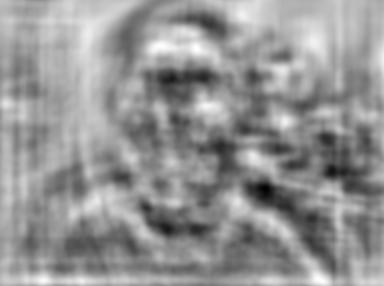
\includegraphics[width=\textwidth]{plots/C_log_SE2_conv.jpg}
        \caption{$C_{\text{log}}^{SE(2)}$}%
        
        \label{fig:mean and std of net44}
    \end{subfigure}
    \hspace{-1\baselineskip}
    \quad
    \begin{subfigure}[b]{0.1\textwidth}   
        \centering 
        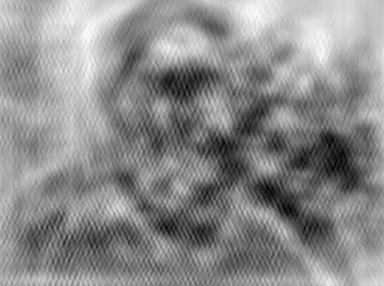
\includegraphics[width=\textwidth]{plots/D_log_SE2_conv.jpg}
        \caption{$D_{\text{log}}^{SE(2)}$}%
        
        \label{fig:mean and std of net44}
    \end{subfigure}
    \hspace{-1\baselineskip}
    \quad
    \begin{subfigure}[b]{0.1\textwidth}   
        \centering 
        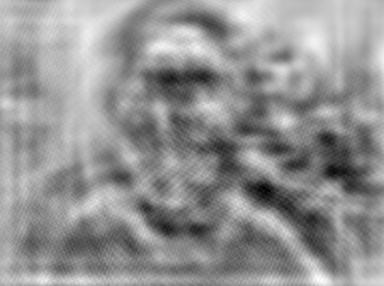
\includegraphics[width=\textwidth]{plots/E_log_SE2_conv.jpg}
        \caption{$E_{\text{log}}^{SE(2)}$}%
        
        \label{fig:mean and std of net44}
    \end{subfigure}

    {\small (b)}

    \caption[ The average and standard deviation of critical parameters ]
    {\small Exemples de templates et leur réponse} 
    \label{fig: template}
\end{figure*}

La figure \ref{fig: template} représente (a) l'image test (b) les différents templates de $\mathbb{R}^2$ que nous avons obtenus sur la première ligne ainsi que leur réponse dans les différents 
cas considérés sur la seconde ligne (b) le maximum d'intensité du template à travers les orientations $\theta$ ainsi que la réponse du template à l'image test.

\paragraph{Influence de la régularisation}

Nous avons voulu rendre compte de l'influence des différents paramètres de régularisation sur la précision du modèle.
Pour ce faire nous avons reporté les valeurs de précision des modèles $C_{\text{lin}}^{SE(2)}$ et $D_{\text{lin}}^{SE(2)}$
en faisant varier les valeurs de $\mu$ et $\lambda$. Les résultats sont visibles en \ref{fig:param}. Cette courbe permet de bien rendre 
compte de l'importance de la régularisation dans un tel problème de détection.

\paragraph{Influence du critère de précision}
Afin d'être tout à fait transparents sur la précision des modèles développé nous avons testé le modèle démontrant les meilleurs 
résultats $C_{\text{lin}}^{SE(2)}$ avec différents valeur de rayon de détection variant de $2$ pixels à $50$ pixels. Les résultats 
peuvent être appréciés en \ref{fig:radius}. Pour un rayon de détection de 2 pixels, la précision du modèle tombe à $37 \%$. Ceci n'est pas 
étonnant dans la mesure où 2 pixels rentre largement dans la gamme de précision de ``labélisation''. Par contre, pour un rayon de détection de 5 pixels, 
le modèle démontre une précision assez bonne de 81 \%, ce qui est en lien avec la valeur précédemment observée pour 10 pixels. Dés que le rayon dépasse 
15 pixels, la précision du modèle stagne. Ceci laisse apercevoir que 10\% des détections sont aberrantes.

\begin{figure}[t]
\centering
\hspace*{-5em}%
\begin{subfigure}{.6\textwidth}
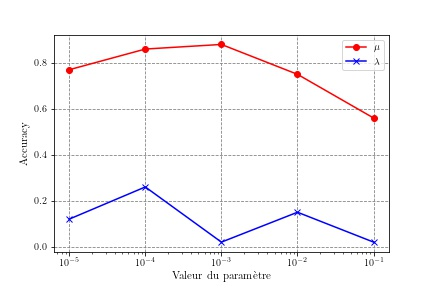
\includegraphics[scale=0.65]{plots/parameter_score_C_D_lin_R2.jpg}%
  \caption{$ \quad \quad \quad $Influence des paramètres de régularisation}%
    \label{fig:param}
\end{subfigure}%
%\hspace*{5em}
\begin{subfigure}{.6\textwidth}
  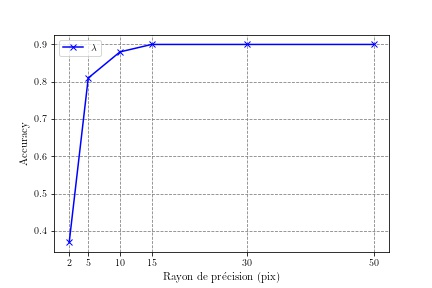
\includegraphics[scale=0.65]{plots/radius_scores.jpg}
  \caption{ Précision en fonction du rayon de détection}%
  \label{fig:radius}
\end{subfigure}
\end{figure}

\vspace{10em}
\paragraph{robustesse au changement d'échelles}\label{paragraph:robustness-to-scale}
Bien que par construction la méthode proposée gère bien les transformations par translation, nous 
avons observé qu'elle n'est pas très robuste aux changements d'échelle comme peut en témoigner la 
figure \ref{fig:zoom}. Dans, cette expérience nous avons utilisé le meilleur modèle obtenu via le méthode 
$C_{\text{lin}}^{SE(2)}$ (c.f. \ref{part:expe}). Nous lui avons demandé de prédire la localisation de la pupile de l'oeil 
gauche sur la même image mais avec des niveaux de zooms différents (x1, x1.5, x2 et x3). La méthode démontre 
une bonne capacité de prédiction pour des facteurs d'échelle assez faible puisse en témoigner l'image zoomée 
x1.5. Cependant, dès lors que le facteur d'échelle dépasse 2, le modèle n'est plus en mesure de prédire correctement 
la localisation de la pupile.  

\begin{figure}[htpb]
    \centering
    %\hspace*{-5em}%
    \begin{subfigure}[b]{0.3\textwidth}
    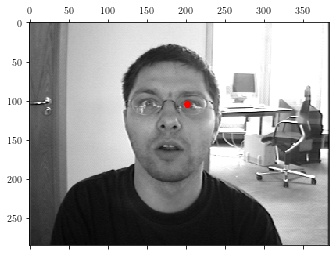
\includegraphics[scale=0.4]{plots/zoom_1.jpeg}%
      \caption{Image original}%
        \label{fig:param}
    \end{subfigure}%
    \quad
    \begin{subfigure}[b]{0.3\textwidth}
      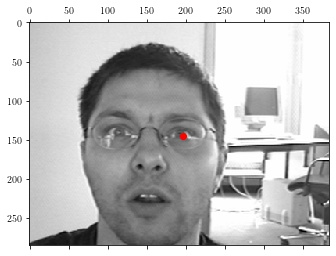
\includegraphics[scale=0.4]{plots/zoom_1_5.jpeg}
      \caption{Zoom x1.5}%
      \label{fig:radius}
    \end{subfigure}
    \vskip\baselineskip
    \begin{subfigure}[b]{0.3\textwidth}
        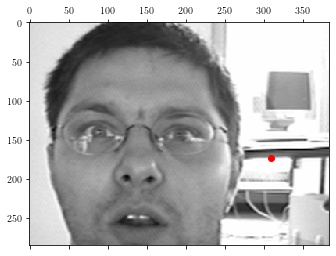
\includegraphics[scale=0.4]{plots/zoom_2.jpeg}
        \caption{Zoom x2}%
        \label{fig:radius}
      \end{subfigure}
      \quad
      \begin{subfigure}[b]{0.3\textwidth}
        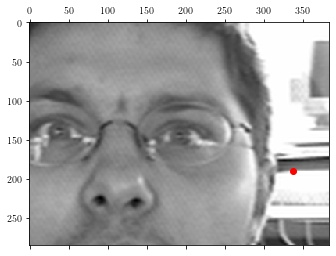
\includegraphics[scale=0.4]{plots/zoom_3.jpeg}
        \caption{Zoom x3}%
        \label{fig:radius}
      \end{subfigure}
      \caption{Même image zoomée et résultat de prédiction}
      \label{fig:zoom}
    \end{figure}


\pagebreak

\begin{thebibliography}{9}

	\bibitem{main}
    Bekkers, E. J., Loog, M., ter Haar Romeny, B. M., \& Duits, R. (2017).
    \emph{Template matching via densities on the roto-translation group.}
    IEEE transactions on pattern analysis and machine intelligence, 40(2), 452-466.
    \bibitem{bspline}
    Thévenaz, P., Blu, T., \& Unser, M. (2000). \emph{Interpolation revisited} [medical
    images application]. IEEE Transactions on medical imaging, 19(7), 739-758.
    \bibitem{orientation-score}
    Bekkers, E., Duits, R., \& Loog, M. (2015, January). \emph{Training of templates for
      object recognition in invertible orientation scores: application to optic nerve
    head detection in retinal images.}
    In International Workshop on Energy Minimization Methods in Computer Vision and Pattern Recognition (pp. 464-477). Springer, Cham.
    \bibitem{cake2}
    Duits, R., Felsberg, M., Granlund, G., \& ter Haar Romeny, B. (2007).
    \emph{Image analysis and reconstruction using a wavelet transform constructed from a
    reducible representation of the Euclidean motion group.} International Journal of Computer Vision, 72(1), 79-102.
    \bibitem{cake}
    Kalitzin, S. N., Romeny, B. M. T. H., \& Viergever, M. A. (1999).
    \emph{Invertible apertured orientation filters in image analysis.}
    International Journal of Computer Vision, 31(2-3), 145-158.
    \bibitem{cross-correlation}
    Yoo, J. C., \& Han, T. H. (2009).
    \emph{Fast normalized cross-correlation.} Circuits, systems and signal processing, 28(6), 819.
    \bibitem{preprocessing}
    Foracchia, M., Grisan, E., \& Ruggeri A. (2005). \emph{Luminosity  and  contrast  normalization  inretinal images}.
    MEDIA, vol. 9, no. 3, pp. 179–90.
\end{thebibliography}

        
\end{document}
 
